\documentclass[10pt,a4paper]{article}
\usepackage[bindingoffset=0.2in,%
            left=2.5cm,right=2cm,top=2.7cm,bottom=1in,%
            footskip=.25in]{geometry}
\usepackage[utf8]{inputenc}
\usepackage[ngerman]{babel}
\usepackage{amsmath, amsfonts, amssymb}
\usepackage{scrpage2}
\usepackage{color}
\usepackage{titlesec}
\pagestyle{scrheadings}
\usepackage{ulem, contour}
\usepackage{hyperref}
\usepackage{pdfpages}
\usepackage{tabularx}
\usepackage{subcaption, float}
\usepackage{scrextend}
\usepackage{enumerate, enumitem}
\usepackage[bottom, splitrule]{footmisc}
\usepackage{multirow, multicol}
\usepackage{csquotes}

\usepackage[style=authoryear, backend=biber]{biblatex}
\addbibresource{bibliography.bib}

\renewcommand{\ULdepth}{1.8pt}
\contourlength{0.8pt}

\newcommand{\cul}[1]{%
  \uline{\phantom{#1}}%
  \llap{\contour{white}{#1}}%
}

\graphicspath{
    {Images/}
}

\makeatletter
\newcommand*{\rom}[1]{\expandafter\@slowromancap\romannumeral #1@}
\makeatother

\newrobustcmd*{\parentexttrack}[1]{%
  \begingroup
  \blx@blxinit
  \blx@setsfcodes
  \blx@bibopenparen#1\blx@bibcloseparen
  \endgroup}

\AtEveryCite{%
  \let\parentext=\parentexttrack%
  \let\bibopenparen=\bibopenbracket%
  \let\bibcloseparen=\bibclosebracket}

\definecolor{gray}{rgb}{0.33, 0.33, 0.33}
\definecolor{greengreen}{rgb}{0.0, 0.56, 0.0}
\definecolor{fgreen}{rgb}{0.13, 0.55, 0.13}
\definecolor{grellow}{rgb}{0.68, 1.0, 0.18}
\definecolor{orange}{rgb}{1.0, 0.49, 0.0}
\definecolor{deepblue}{rgb}{0,0,0.5}
\definecolor{deepred}{rgb}{0.6,0,0}
\definecolor{deepgreen}{rgb}{0,0.5,0}

\usepackage{pifont}

\newcommand{\cmark}{\ding{51}}%
\newcommand{\xmark}{\ding{55}}%
\newcommand{\wontfix}{\rlap{$\square$}{\large\hspace{1pt}\xmark}}


\newcommand{\vnr}{32}
\newcommand{\anr}{1}

\ihead{}
\ohead{Anfängerpraktikum 2}
\chead{Versuch \vnr, Abgabe \anr : Dielektrizitätskonstante}
\cfoot{\pagemark}
\setheadsepline{.5pt}
\setlength\parindent{0pt}

\begin{document}

\begin{multicols}{2}
\begin{labeling}{Versuch-Nr.:}
\item[\textcolor{white}{x}Protokollant:\hspace{38pt}] \cul{Name} \wontfix
\item[\textcolor{white}{x}Zusammenarbeit\footnotemark mit:] \cul{Name} $\square$
\item[\textcolor{white}{x}Datum:\hspace{62pt}] \cul{\today}

\columnbreak

\item[Kurs: \hspace{27pt}] \cul{Anfängerpraktikum 2}
\item[Assistent: \hspace{8.7pt}] \cul{Name}
\item[Versuch-Nr.:] \underline{\vnr}
\end{labeling}
\end{multicols}

\begin{figure}[h]
\hspace{-0.5cm}\centerline{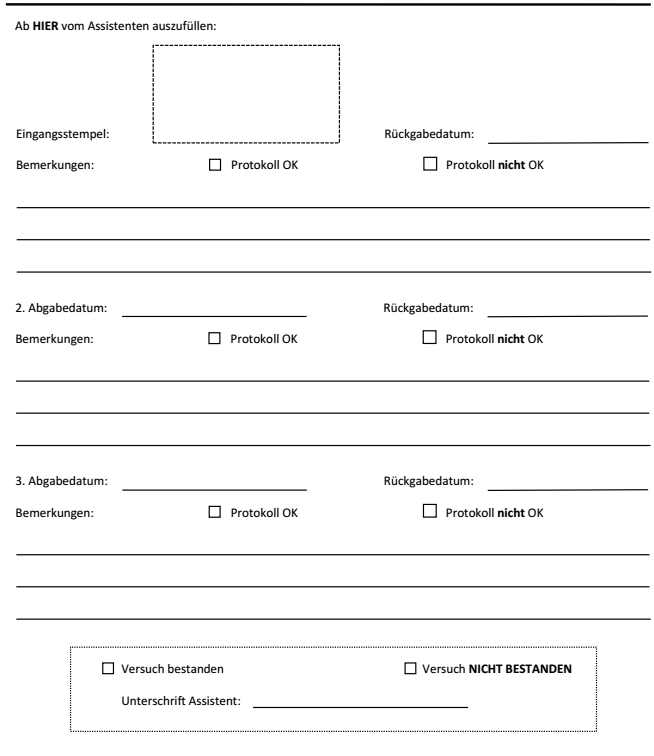
\includegraphics[width=1.1\linewidth , height=19cm]{Deckblatt_rest}}
\end{figure}

\newpage

\tableofcontents

\vspace{10pt}


\section{Aufgabenstellung}
\begin{flushleft}
Der Versuch \vnr \vspace{1pt} behandelt das Ermitteln der Dielektrizitätskonstante (bzw. Permittivität) im Experiment.
\end{flushleft}

\subsection{Physikalischer Hintergrund}
\begin{flushleft}
Die Permittivität gibt die Polarisationsfähigkeit eines Materials durch elektrische Felder an\footnote{Quelle: \href{https://de.wikipedia.org/wiki/Permittivit\%C3\%A4t}{Wikipedia}}. Dabei bezeichnet die naturkonstante $\varepsilon_0$ die Permittivität von Vakuum. Die Permittivität aller Stoffe wird als ein Vielfaches dieser Konstanten angegeben mit $\varepsilon = \varepsilon_r \cdot \varepsilon_0$ und $\varepsilon_r$ als relative Permittivität.
\end{flushleft}
\begin{flushleft}
Wir bestimmen die Permittivität mit Hilfe von Kondensatoren. Hierbei ist diese\footnote{(bei Plattenkondensatoren - die wir verwenden)} mit der Kapazität verbunden durch
\begin{equation}\label{eq:kapaz}
C = \frac{U}{Q} = \varepsilon \frac{A}{d}
\end{equation}
Der Zusammenhang zeigt also, dass die Kapazität mit der Permittivität zusammenhängt, d.h. der Kondensator im Vakuum besitzt eine andere Kapazität, als in Wasser oder, wenn beispielsweise Papier zwischen den Platten befindlich ist\footnote{Vakkuum: $\varepsilon_{r,Vakuum} = 1$, sonst: $\varepsilon_r > \varepsilon_{r,Vakuum}$}.
\begin{equation}\label{eq:kapa_relp}
C = \varepsilon_r \cdot \varepsilon_0 \cdot \frac{A}{d}
\end{equation}
\end{flushleft}
\subsubsection{Berechnung der Permittivität \label{sec:herl}}
\begin{flushleft}
Wir wollen nun zunächst die Gleichung zur Berechnung der Permittivität herleiten. Für unser Experiment nutzen wir einen \textit{elektromagnetischen Schwingkreis} (mehr dazu später) und wollen diesen in den Resonanzfall versetzen (bzw. halten). Damit dies geschieht, müssen die Frequenzen des Schwingkreises und eines Senders von außen (Entgegenwirken der Dämpfung) übereinstimmen.
\begin{align}
f_{Sender} &= f_{Schwing} \label{eq:freq_eq}\\
2 \pi \sqrt{L_{Sender} \cdot C_{Sender}} &= 2 \pi \sqrt{L_{Schwing} \cdot C_{Schwing}} \label{eq:t_eq}\\
C_{Sender} &= C_{Schwing} \label{eq:c_eq}
\end{align}
Für Gleichung \ref{eq:c_eq} muss dabei aber gelten $L_{Sender} = L_{Schwing}$.
\end{flushleft}
\begin{flushleft}
Für die Messungen in diesem versuch ist es nun notwendig, die Kapazität des Schwingkreises zu eichen, sodass wir auch tatsächlich den Resonanzfall herstellen und Gleichung \ref{eq:c_eq} gilt. Dazu Schalten wir in den Empfängerkreis einen Kondensator mit bekannter Kapazität $C_{ref}$ ein (Siehe: Abbildung \ref{fig:schalt_resonanz}) und stellen den Drehkondensator im Senderkreis so ein, dass der Empfängerkreis in Resonanz ist (\textit{Indikator}: die Glühbirne leuchtet dann am hellsten). Hierbei notieren wir die Kapazität am Drehkondensator als $C_0 := C_{Dreh}(\phi_0)$. Es gilt die -Gleichheit von Gleichung \ref{eq:c_eq}.
\end{flushleft}
\begin{flushleft}
Nach dam Eichen kann nun der Tauchkondensator (in Luft) eingeschalten werden (Abbildung \ref{fig:schalt_sender}). Dadurch erhöht sich die Gesamtkapazität, die nun mit dem Drehkondensator wieder justiert werden muss. Im REsonanzfall haben wir dann wieder Gleichung \ref{eq:c_eq} erfüllt und können berechnen:
\begin{align}
C_{Sender} = C_{Empfaenger} = C_0 &= C_{Dreh}(\phi_{luft}) + C_{tauch} \label{eq:cs=cd+ct} \\
C_{tauch} &= C_0 - \underbrace{C_{luft}}_{C_{Dreh}(\phi_{luft})} \label{eq:ctauch}
\end{align}
Als nächstes tauchen wir den Tauchkondensator in Öl ein und stellen den Drehkondensator wieder ein.
\begin{equation}\label{eq:tauchinoel}
C_{Sender} = C_{Empfaenger} = C_0 = C_{Dreh}(\phi_{oel}) + \varepsilon \cdot C_{tauch}
\end{equation}
Wir setzen nun Gleichung \ref{eq:ctauch} in Gleichung \ref{eq:tauchinoel} ein:
\begin{align}
C_0 &= C_{oel} + \varepsilon \cdot (C_0 - C_{luft}) \\
\varepsilon &= \frac{C_0 - C_{oel}}{C_0 - C_{luft}} \label{eq:epsi_wc}
\end{align}
Wir haben nun die Formel zur Berechnung der Permittivität in diesem Versuch hergeleitet, doch wir können diese Formel noch weiter vereinfachen. Wie bereits klar wurde, arbeiten wir mit einem Drehkondensator, dessen Kapazität wir anhand der Winkeleinstellung bestimmen. Dabei hängt die Kapazität vom Winkel $\phi$ anhand einer linearen Funktion ab:
\begin{equation}
C_{Dreh} = a \cdot \phi + b
\end{equation}
Wir können die hergeleitete Formel nun weiterrechnen:
\begin{align}
\varepsilon &= \frac{C_0 - C_{oel}}{C_0 - C_{luft}} \nonumber \\
\varepsilon &= \frac{a \cdot \phi_0 + b - (a \cdot \phi_{oel} + b)}{a \cdot \phi_0 + b - (a \cdot \phi_{luft} + b)} \nonumber \\
\varepsilon &= \frac{\phi_0 - \phi_{oel}}{\phi_0 - \phi_{luft}}
\end{align}
Wir können somit also die Permittivität durch den Winkel am Drehkondensator bestimmen.
\end{flushleft}

\section{Messmethoden}
\begin{flushleft}
In diesem Versuch wollen wir einen \textbf{elektromagnetischen Schwingkreis} nutzen, um die Kapazitäten - und daraus die Permittivität - zu bestimmen. Dazu bauen wir zwei Schwingkreise auf, einen \textbf{Senderschwingkreis} und einen \textbf{Empfängerschwingkreis}. Zweiterer wird zu einem \textbf{Resonanzschwingkreis}, der über den \textit{Senderschwingkreis} im Resonanzfall gehalten wird (Siehe: Abbildung \ref{fig:schalts} (Schaltbilder)).
\end{flushleft}

\subsection{Versuchsaufbau}
\begin{flushleft}
Für diesen Versuch benötigen wir
\begin{itemize}[itemsep=0pt]
\item Eine Spannungsquelle
\item Zwei Spulen (mit gleicher Induktivität $L$)
\item Ein Drehkondensator
\item Ein Tauchkondensator
\item Eine Lampe (als Indiktor zur Erkennung der Resonanz)
\item Ein Tauchbecken für den Tauchkondensator; Pflanzliches Öl
\end{itemize}
Zusätzlich werden natürlch Kabel benötigt, um alles zu verbinden. Des weiteren schalten wir noch einen Hochvolt-Schalt-Transistor mit Schutzschaltung ein (Abbildung \ref{fig:transistor}).
\end{flushleft}

\subsection{Schaltbilder}
\begin{flushleft}
\begin{figure}[H]
\centering
\begin{subfigure}[t]{.5\textwidth}
\centering
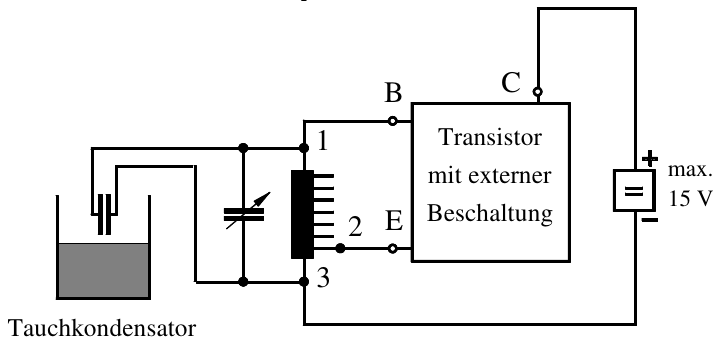
\includegraphics[scale=0.4]{schalt_sendkreis}
\subcaption{Schaltbild des Sendekreises.}
\label{fig:schalt_sender}
\end{subfigure}%
%
\begin{subfigure}[t]{.5\textwidth}
\centering
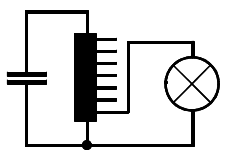
\includegraphics[scale=0.4]{schalt_reskreis}
\subcaption{Schaltbild des Sendekreises.}
\label{fig:schalt_resonanz}
\end{subfigure}%
\caption{Schaltbilder des Sende- und Resonanzkreises.\protect\footref{foot:imgsrc}}
\label{fig:schalts}
\end{figure}

\begin{figure}[H]
\centering
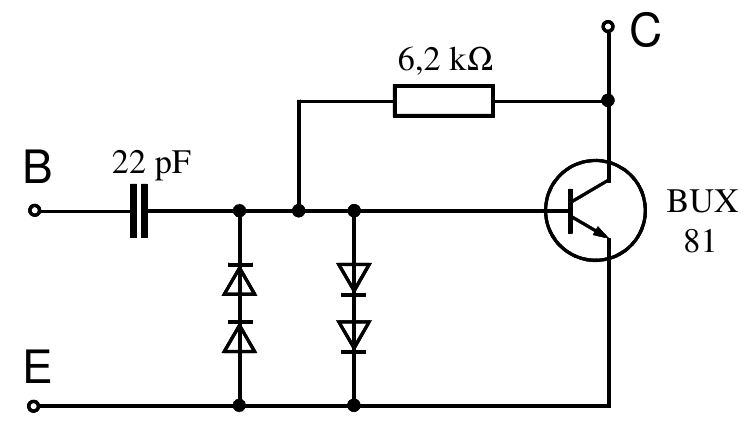
\includegraphics[scale=0.4]{schalt_trans}
\caption{Schaltbild des Hochvolt-Schalt-Transistors mit Schutzschaltung.\protect\footnotemark}
\label{fig:transistor}
\end{figure}
\footnotetext{Bilderquelle: \href{https://www.uni-frankfurt.de/49295015/Generic_49295015.pdf}{Versuchsanleitung zu Versuch 32} des Anfängerpraktikum \rom{2}, Institut für Angewandte Physik, Goethe-Universität Frankfurt a. M. \label{foot:imgsrc}}
\end{flushleft}

\section{Versuchsdruchführung}
\begin{flushleft}
\textit{Hinweis}: In der Herleitung der Formel zur Berechnung der Permittivität (Abschnitt \ref{sec:herl}) ist der Ablauf des Versuches bereits beschrieben.
\end{flushleft}
\begin{flushleft}
Wir beginnen, indem wir die beiden Kreise aus den Schaltbildern (Abbildung \ref{fig:schalts}) aufbauen. Danach können wir den Schwingkreis eichen, damit unsere hergeleiteten Formeln gelten. Dazu schalten wir den Tauchkondensator noch nicht in den schwingkreis ein, lediglich den Vergleichskondensator $C_{ref}$ in den Empfängerkreis. Wir stellen nun den Drehkondensator ein, sodass ein Resonanzkreis entsteht (Empfängerkreis $\to$ Resonanzkreis) - der Punkt an dem die Lampe am hellsten leuchtet. Wir notieren den Winkel am Drehkondensator als $\phi_0$.

Als nächstes schalten wir den Tauchkondensator ein (behalten in aber in Luft) und justieren den Drehkondensator, sodass wieder der Resonanzkreis steht. Wir notieren diesen winkel des Drehkondensators als $\phi_{luft}$.

Zum Schluss machen wir das gleiche mit dem tauchkondensator in Öl getaucht. Dieser Wert des Drehkondensators ist $\phi_{oel}$.
\end{flushleft}
\begin{flushleft}
Wir bestimmen diese Winkel für drei verschiedene Vergleichskondensatoren und notieren die Ergebnisse.
\end{flushleft}

\section{Versuchsergebnisse}
\begin{flushleft}
\begin{table}[H]
\centering
\caption{Messergebnisse der Winkel am Drehkondensator.}
\label{tab:messerg}
\begin{tabular}{|c|c|c|c|c|c|c|}
\hline
\textbf{$C_{ref} [pF]$} & \textbf{$\phi_0 [^{\circ}]$} & \textbf{$\phi_{luft} [^{\circ}]$} & \textbf{$\phi_{oel} [^{\circ}]$} & \textbf{$\Delta \phi [^{\circ}]$} & \textbf{$\varepsilon$} & \textbf{$\Delta \varepsilon$} \\
\hline
780 & 152 & 125.5 & 59 & 5 & 3.51 & 0.378 \\ 
\hline
560 & 94.5 & 67.5 & 6.5 & 5 & 3.26 & 0.371 \\ 
\hline
680 & 124.5 & 99.5 & 33.5 & 5 & 3.64 & 0.4 \\ 
\hline
\end{tabular}
\end{table}
Die Tabelle \ref{tab:messerg} zeigt die Messergebnisse der Winkel am Drehkondensator\footnote{Wir verwenden hier $\Delta \phi = 5^{\circ}$, da der tatsächliche Fehlerrahmen nicht angegeben ist. Die $5^{\circ}$ sollten aber eine gute Fehlerabdeckung sein.}, sowie die berechneten Werte für die Permittivität. Aus diesen Werten bestimmen wir den Mittelwert:
\begin{figure}[H]
\centering
\begin{subfigure}[c]{0.5\textwidth}
\subcaption{Berechnung des Mittelwertes}
\begin{align*}
\varnothing \varepsilon &= \frac{1}{n} \sum \varepsilon_i \\
&\approx \frac{10.40869}{3} \\
&\approx 3.47 \\
\end{align*}
\end{subfigure}%
\begin{subfigure}[c]{0.5\textwidth}
\subcaption{Berechnung des Standardfehlers}
\begin{align*}
\sigma_{\bar{x}} &= \frac{\sigma}{\sqrt{n}} = \sqrt{\frac{\sum(\varepsilon_i - \varnothing \varepsilon)^2}{n-1}} \cdot \frac{1}{\sqrt{n}} \\
&= \frac{0.1934754512}{\sqrt{3}} \\
&\approx 0.11
\end{align*}
\end{subfigure}%
\end{figure}
Wir haben somit die Permittivität des pflanzlichen Öls bestimmt, mit $\varepsilon \approx 3.47 \pm 0.11$.
\end{flushleft}

\section{Diskussion der Messergebnisse}
\begin{flushleft}
Wir haben die Permittivität bestimmt und können daran nun ermitteln, welches Öl verwendet worden sein könnte. Es kommen folgende Substanzen in betracht\footnote{\href{https://www.vega.com/-/media/PDF-files/Dielektrizitaetszahl-Liste_DE.pdf}{Quelle} (es wurden nur pflanzliche Substanzen betrachtet)}.
\begin{itemize}[itemsep=0pt]
\item Raps ($\varepsilon = 3.3$)
\item Isosafrol ($\varepsilon = 3.3$)
\item Rübensamen ($\varepsilon = 3.5$)
\end{itemize}
Wir sehen also, dass unser Ergebnis der Permittivität des verwendeten Öls um mehr als den berechneten Fehler $\Delta \varepsilon$ abweichen kann. Die tatsächliche Permittivität ist jedoch nicht bekannt.
\end{flushleft}

\section{Fazit}
\begin{flushleft}
Der Versuch \vnr\vspace{1pt} hat gezeigt, dass ein Versuch nicht unbedingt ausreicht, um etwas zu ermitteln - in diesem Versuch konnten wir das verwendete Öl nicht konkret bestimmen.
\end{flushleft}

\begingroup
\raggedright
\sloppy
\printbibliography[heading=bibintoc,title={6 \hspace{6pt} Literatur}]
\endgroup

\end{document}